% Input-ready appendix additions for the main paper.
% Assumes the main paper already loads: graphicx, float, listings.
% Assumes the main paper bibliography includes the entry jin2025sysmbench.

\noindent
These appendix additions summarize selected follow-on analyses over 151 SysMBench prompts and four model backends (604 total model-prompt runs). Because eventual syntactic success reaches 100\% under iterative repair in this campaign, the more informative appendix-level outcomes are iterations-to-success and adjacent-iteration repair behavior.

\section{Extended Analysis: Difficulty and Output-Length Signals}
This appendix section examines whether iteration count is meaningfully related to either the SysMBench difficulty label or the length of the generated SysML output. The purpose is to test whether repair effort is primarily a size-driven phenomenon.

\subsection{SysMBench Difficulty Versus Iterations-to-Success}
In this first analysis, we use the SysMBench difficulty classification~\cite{jin2025sysmbench}. In their scheme, each prompt is assigned a difficulty bucket from the line count of the hand-authored ground truth SysML model, not from the generated output. The bucket definitions are: difficulty 1 for fewer than 30 lines, difficulty 2 for 30--59 lines, difficulty 3 for 60--89 lines, difficulty 4 for 90--119 lines, and difficulty 5 for 120 or more lines. Across the 151 benchmark prompts, this yields \(n=63, 64, 12, 6,\) and \(6\) prompts in difficulty buckets 1 through 5, respectively. Because each prompt is evaluated with four models, the pooled right-panel averages in Figure~\ref{fig:appendix_difficulty} are computed from 252, 256, 48, 24, and 24 prompt-model cases across the five difficulty levels. Figure~\ref{fig:appendix_difficulty} tests whether that benchmark-defined size proxy tracks repair effort in the validator-in-the-loop setting.

\begin{figure}[!t]
\centering

\includegraphics[width=\columnwidth,keepaspectratio]{appendix/appendix_additions/figures/fig09_difficulty_mean_iterations_to_success_grouped_bar.png}
\caption{Difficulty-conditioned repair effort with model split and pooled trend. The pooled mean iterations-to-success are 1.766, 1.668, 1.938, 1.667, and 1.583 for difficulty levels 1 through 5, respectively, with a pooled linear fit of \(R^2 \approx 0.183\).}
\label{fig:appendix_difficulty}
\end{figure}

The pooled mean iterations-to-success are 1.766, 1.668, 1.938, 1.667, and 1.583 across difficulty levels 1 through 5, respectively. The weak linear fit indicates that the hand-authored ground truth SysML line-count difficulty label is not strongly correlated with repair effort, as measured here by iterations-to-success.

\subsection{Generated Output Length Versus Iterations-to-Converge}
Since SysMBench difficulty is line-count based, and one might reasonably expect repair effort to increase with the number of lines generated, it is useful to ask whether the length of the \emph{generated} SysML output is itself correlated with iterations-to-converge.

\begin{figure}[H]
\centering
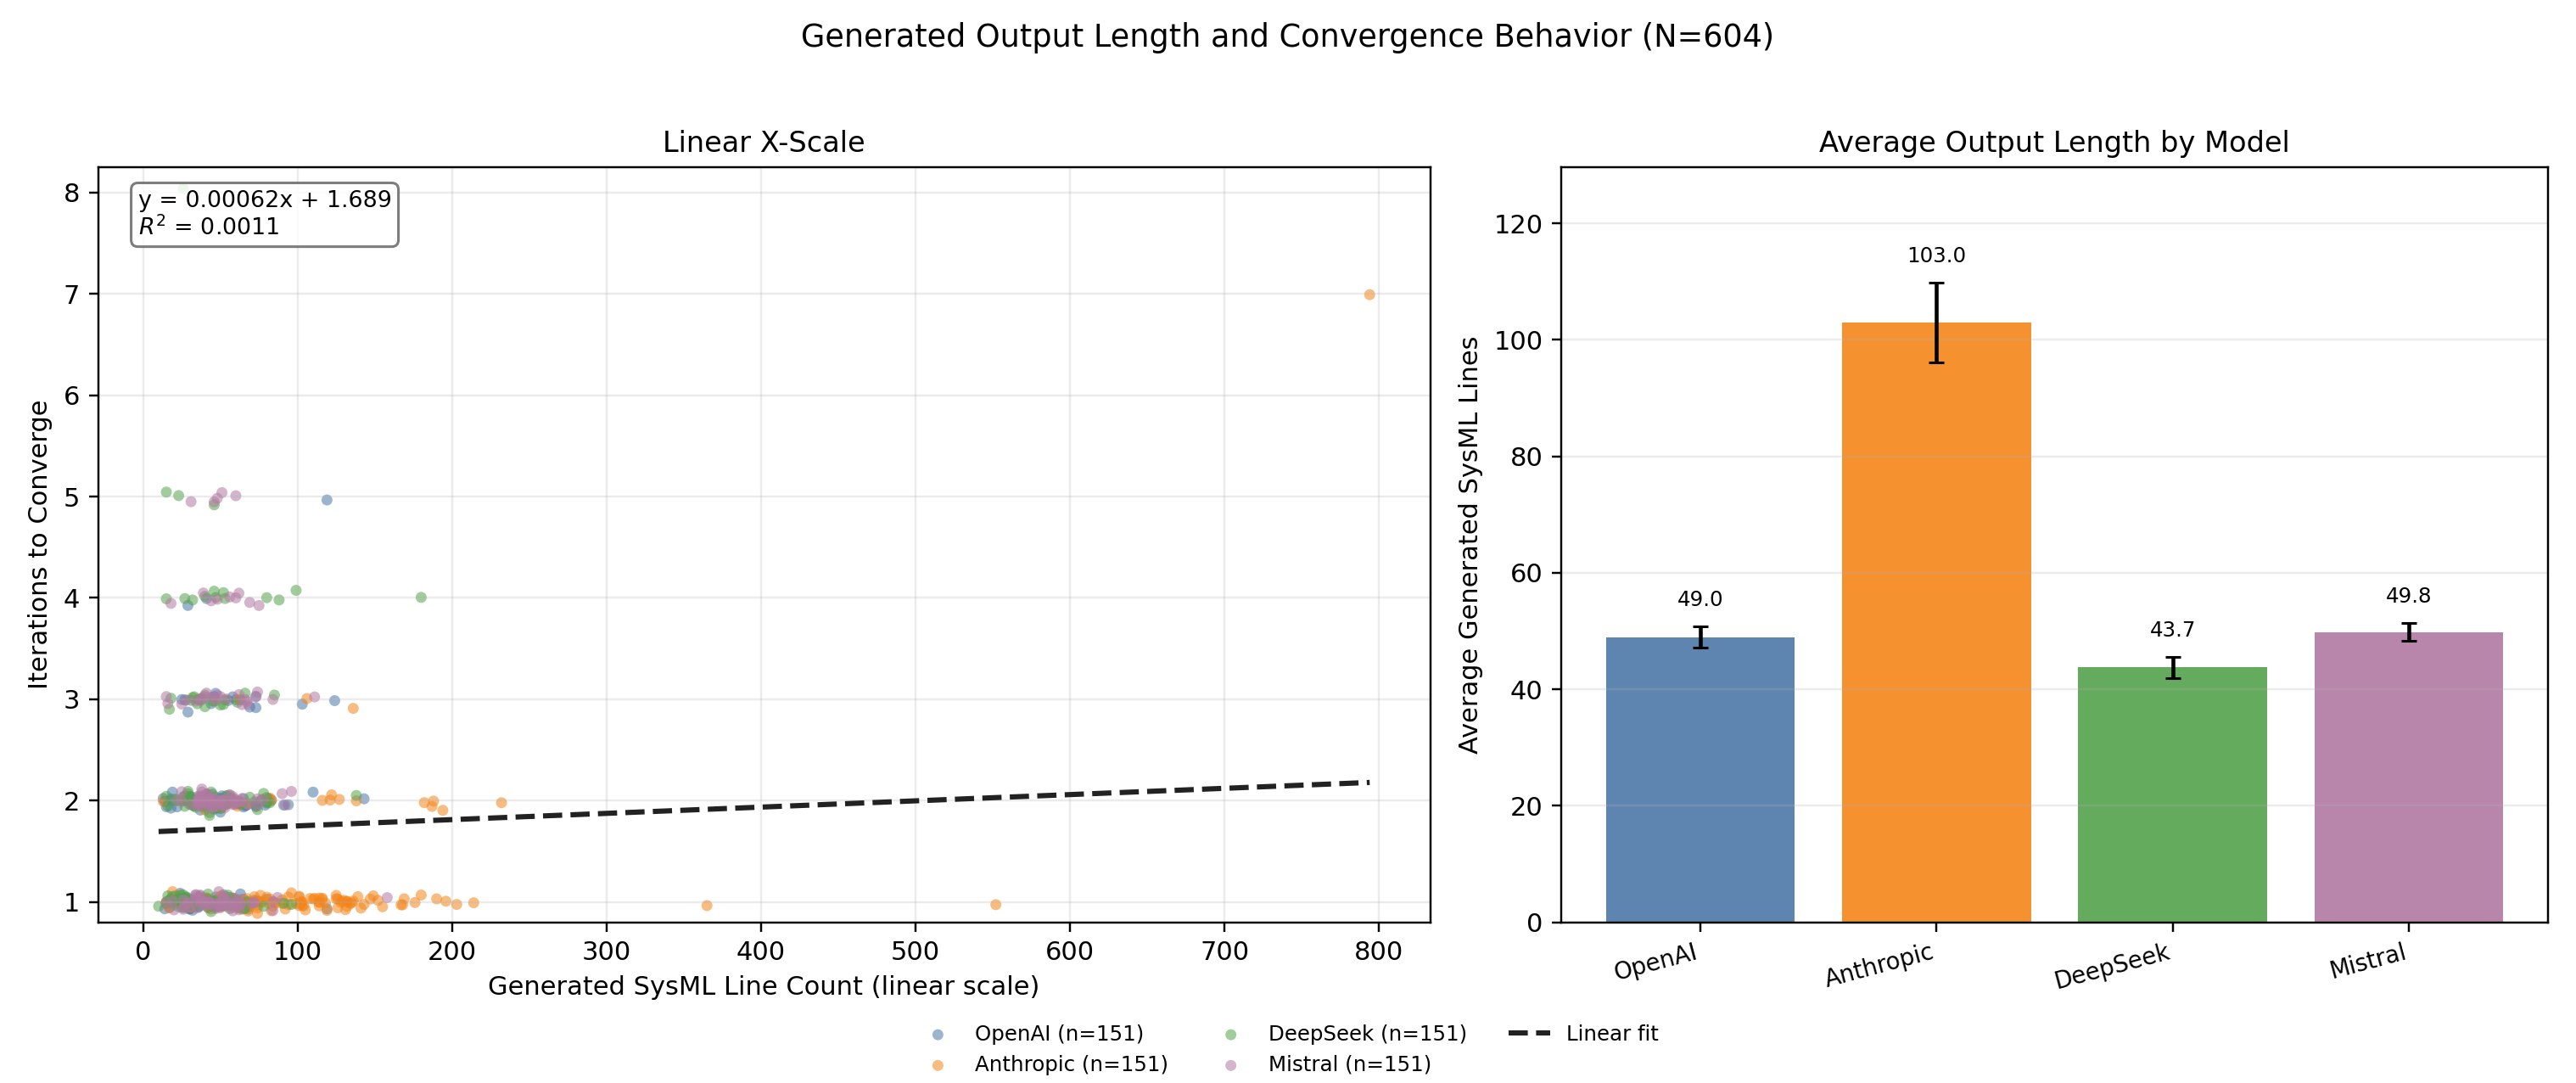
\includegraphics[width=\columnwidth,keepaspectratio]{appendix/appendix_additions/figures/fig14_generated_output_lines_vs_iterations_scatter_trend.png}
\caption{Generated SysML output length analysis. The left panel shows a scatter plot of generated SysML line count versus iterations-to-converge, with the pooled linear fit overlaid (\(R^2 = 0.0011\), slope \(= 0.00062\)). The right panel shows the average generated SysML line count for each model, with error bars indicating standard error.}
\label{fig:appendix_generated_lines}
\end{figure}

The pooled linear fit in Figure~\ref{fig:appendix_generated_lines} is essentially flat (\(R^2 = 0.0011\), slope \(= 0.00062\)), which indicates that generated SysML line count explains almost none of the variation in iterations-to-converge. In this analysis, generated output length is therefore not strongly correlated with repair effort.

The model-level averages in the right panel reinforce the same point. OpenAI, DeepSeek, and Mistral produce broadly similar output lengths on average (approximately 49, 44, and 50 lines, respectively), whereas Anthropic produces about 103 lines on average, or roughly twice as many. However, Anthropic also required the fewest iterations-to-success on average in the main results (1.23, versus 1.73 for OpenAI, 1.97 for DeepSeek, and 1.98 for Mistral), further indicating that line count alone is a poor standalone proxy for repair effort. Taken together, Figures~\ref{fig:appendix_difficulty} and~\ref{fig:appendix_generated_lines} suggest that repair effort is not well explained by size alone.

One possible explanation is that raw line count does not necessarily reflect the number of distinct syntactic structures that must be formed correctly. A model can generate many lines by expanding a relatively uniform pattern, whereas a shorter output may still involve a wider variety of declarations, references, and nested relationships that are more sensitive to validator failure. Simply producing more lines of the same structure therefore need not imply greater repair effort.

\section{Extended Analysis: Classifying Repair Attempts on Persistent Errors}
This appendix section looks at what the LLM does from one iteration to the next when a persistent error is still present. We treat an error as \emph{persistent} if an identical SysIDE diagnostic, meaning the same error family and the same \texttt{stderr} message, appears in two consecutive iterations of the same prompt-model run. To study the repair attempt itself, we compare the SysML artifact from iteration \(k\), which is the previous attempt fed back into the loop, with the revised SysML artifact produced by the LLM at iteration \(k+1\).

\subsection{Error Transition Outcome Explanations}
Using the SysIDE \texttt{stderr} outputs, we ask a simple question: when an identical error is still present at iteration \(k+1\), did the LLM appear to change the highlighted failing region, or did it leave that region unchanged? Across all back-to-back iteration pairs, this yields 1502 exact-error transitions. Each transition corresponds to one exact SysIDE diagnostic observed at iteration \(k\) and checked again at iteration \(k+1\). This is smaller than the total number of raw error instances because repeated copies of an identical SysIDE message within a single iteration are collapsed into one signature-level transition event. That choice is intentional: here we want to measure whether the model corrected an error pattern from one iteration to the next, not whether it repaired every repeated occurrence independently. We interpret many repeated identical grammar diagnostics as manifestations of the same underlying structural issue, so once the model applies the relevant pattern-level fix, repeated instances will often be corrected together rather than one by one.

Of these 1502 transitions, 1262 are resolved by the next iteration and are therefore not persistent. The remaining 240 persist through the next repair attempt. These 240 persistent transitions are the cases for which we want to understand whether the model tried to repair the highlighted region but failed, or whether it effectively carried the same failing code forward unchanged.

We then classify the 240 persistent cases into one of two categories:
\begin{itemize}
    \item \textbf{Unaddressed and not fixed}: an identical validator error remains at iteration \(k+1\), and the validator highlights an identical code snippet again.
    \item \textbf{Addressed but not fixed}: an identical validator error remains at iteration \(k+1\), but the validator now highlights a different code snippet instead, suggesting that the LLM changed the code to attempt to fix the error, but was unsuccessful.
\end{itemize}

To classify these persistent cases, we use the \texttt{stderr} outputs from SysIDE directly. For each persistent identical validator error, we compare the SysIDE \texttt{stderr} block at iteration \(k\) with the corresponding \texttt{stderr} block at iteration \(k+1\), and check whether SysIDE is still highlighting the identical code snippet or now highlights a different snippet instead.

For example, consider the following SysIDE \texttt{stderr} output. For readability, the long expected-token list is abbreviated here, but the full raw message is used in the analysis:
\begin{lstlisting}
iteration_01.sysml:36:19: error (parsing-error):
    Unexpected 'state', expected one of [...]
    36 |         attribute state : VehicleState;
       |                   ^^^^^
\end{lstlisting}
In this example, we classify the transition as ``unaddressed and not fixed'' only if iteration \(k+1\) still contains that identical \texttt{parsing-error} message and still highlights the identical code snippet, \texttt{attribute state : VehicleState;}. If iteration \(k+1\) still contains the identical \texttt{parsing-error} message but SysIDE now highlights a different code snippet instead, we classify the transition as ``addressed but not fixed.'' This is determined directly from validator stderr rather than by manually reading the full file.

A small amount of noise is possible for the ``addressed but not fixed'' category if multiple identical errors occur in different code regions within the same file. In that edge case, the LLM could fix one identical occurrence but fail to fix another identical occurrence on a different code segment, which would still appear here as ``addressed but not fixed.'' We expect this to be uncommon in practice, because many grammar repairs are pattern-level corrections that tend to fix repeated identical structures together.

\subsection{Persistent Error Analysis}
Figure~\ref{fig:appendix_persistent_transition_outcomes} restricts attention to the 240 persistent transitions and shows the split between the two persistent outcomes. Of these persistent cases, 155/240 (64.6\%) are ``unaddressed and not fixed,'' while 85/240 (35.4\%) are ``addressed but not fixed.''

\begin{figure}[H]
\centering
\definecolor{singleShotColor}{RGB}{196,106,28}
\definecolor{pipelineColor}{RGB}{44,138,100}
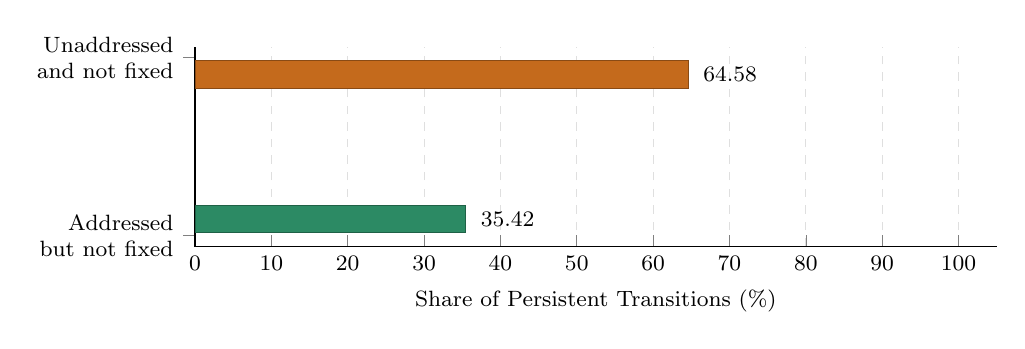
\begin{tikzpicture}
\begin{axis}[
    xbar,
    width=0.97\columnwidth,
    height=0.34\columnwidth,
    xmin=0,
    xmax=105,
    xlabel={Share of Persistent Transitions (\%)},
    symbolic y coords={Addressed,Unaddressed},
    ytick={Unaddressed,Addressed},
    yticklabels={{Unaddressed\\and not fixed},{Addressed\\but not fixed}},
    enlarge y limits={abs=4pt},
    axis lines*=left,
    xmajorgrids=true,
    grid style={dashed,gray!25},
    tick label style={font=\footnotesize},
    yticklabel style={align=right},
    label style={font=\footnotesize},
    nodes near coords={\pgfmathprintnumber[fixed,precision=2]{\pgfplotspointmeta}},
    every node near coord/.append style={font=\footnotesize, text=black, anchor=west, xshift=2pt},
]
\addplot+[fill=singleShotColor, draw=singleShotColor!70!black] coordinates {
    (64.58,Unaddressed)
};
\addplot+[fill=pipelineColor, draw=pipelineColor!70!black] coordinates {
    (35.42,Addressed)
};
\end{axis}
\end{tikzpicture}

\caption{Persistent exact-error outcomes among the 240 transitions for which an identical validator error remains present at iteration \(k+1\). Of these persistent cases, 155/240 (64.6\%) are unaddressed and not fixed, while 85/240 (35.4\%) are addressed but not fixed.}
\label{fig:appendix_persistent_transition_outcomes}
\end{figure}

The larger unaddressed-and-not-fixed share points to an inefficiency in the repair loop. In these cases, SysIDE is still highlighting the identical offending code region in the next iteration, suggesting that the LLM did not change that highlighted region after receiving the validator feedback. This motivates future work on stronger grounding of the prompt to the validator-highlighted snippet, or repair policies that explicitly require the highlighted region to be revised before resubmission.

The addressed-but-not-fixed share instead suggests LLM limitations. In these cases, the model appears to make a repair attempt, but the identical validator error still remains. This suggests a limitation in repair capability rather than simple loop inefficiency: the model changes the code, but does not produce a syntactically valid correction. Future work here should focus on constrained editing or fine-tuning with the large datasets of syntactically valid code that can now be produced. One caveat is that this analysis is based on SysIDE \texttt{stderr} and highlighted snippets, so rare repeated-identical-error cases can still add a small amount of noise.
